\section{Experimentos}
\label{sec:experiments}

\begin{table}
	\caption{Calidad de emboscada para los grafos g1 y g2 utilizando distinto
	n\'umero de agentes (\#) ubicados en posiciones aleatorias distintas (arriba) y
	compartiendo la posici\'on inicial (abajo)}
	\label{tab:ambush_g}
	\centering
	\begin{small}
		\setlength{\tabcolsep}{4pt}
		\begin{tabular}{|c|cc|cc|cc|cc|}
			\hline
			\multicolumn{9}{|c|}{\textbf{g1 (60 pol\'igonos)}}\\
			\hline			
			\multirow{2}{*}{\textbf{\#}} &
			\multicolumn{2}{c|}{\textbf{\astar}} &
			\multicolumn{2}{c|}{\textbf{\ambush}} &
			\multicolumn{2}{c|}{\textbf{P}} &
			\multicolumn{2}{c|}{\textbf{SAR}}\\
			& $\Phi$ & $\Phi^*$ & $\Phi$ & $\Phi^*$&
			$\Phi$ & $\Phi^*$& $\Phi$ & $\Phi^*$\\
			\hline
			2  & 0.71 & 0.73 & 0.82 & 0.84 & 0.82 & 0.84 & 0.83 & 0.84\\
			5  & 0.89 & 0.90 & 0.99 & 1.00 & 0.99 & 1.00 & 0.99 & 1.00\\
			10 & 0.98 & 0.98 & 1.00 & 1.00 & 1.00 & 1.00 & 1.00 & 1.00\\
			20 & 0.97 & 0.99 & 0.98 & 1.00 & 0.98 & 1.00 & 0.98 & 1.00\\
			\hline
			\multicolumn{9}{|c|}{\textbf{g2 (85 pol\'igonos)}}\\
			\hline
			\multirow{2}{*}{\textbf{\#}} &
			\multicolumn{2}{c|}{\textbf{\astar}} &
			\multicolumn{2}{c|}{\textbf{\ambush}} &
			\multicolumn{2}{c|}{\textbf{P}} &
			\multicolumn{2}{c|}{\textbf{SAR}}\\
			& $\Phi$ & $\Phi^*$ & $\Phi$ & $\Phi^*$&
			$\Phi$ & $\Phi^*$& $\Phi$ & $\Phi^*$\\
			\hline
			2  & 0.65 & 0.67 & 0.87 & 0.89 & 0.87 & 0.89 & 0.88 & 0.90\\
			5  & 0.87 & 0.87 & 1.00 & 1.00 & 1.00 & 1.00 & 1.00 & 1.00\\
			10 & 0.95 & 0.95 & 1.00 & 1.00 & 1.00 & 1.00 & 1.00 & 1.00\\
			20 & 0.99 & 0.99 & 1.00 & 1.00 & 1.00 & 1.00 & 1.00 & 1.00\\
			\hline
		\end{tabular}
		
		\bigskip
		\begin{tabular}{|c|cc|cc|cc|cc|}
			\hline
			\multicolumn{9}{|c|}{\textbf{g1 (60 pol\'igonos)}}\\
			\hline			
			\multirow{2}{*}{\textbf{\#}} &
			\multicolumn{2}{c|}{\textbf{\astar}} &
			\multicolumn{2}{c|}{\textbf{\ambush}} &
			\multicolumn{2}{c|}{\textbf{P}} &
			\multicolumn{2}{c|}{\textbf{SAR}}\\
			& $\Phi$ & $\Phi^*$ & $\Phi$ & $\Phi^*$&
			$\Phi$ & $\Phi^*$& $\Phi$ & $\Phi^*$\\
			\hline
			2 & 0.50 & 0.50 & 0.81 & 0.81 & 0.81 & 0.81 & 0.83 & 0.83\\
			5 & 0.48 & 0.48 & 0.97 & 0.98 & 0.97 & 0.98 & 0.97 & 0.98\\
			10 & 0.46 & 0.46 & 0.96 & 0.96 & 0.96 & 0.96 & 0.94 & 0.95\\
			20 & 0.47 & 0.48 & 0.98 & 0.99 & 0.98 & 0.99 & 0.97 & 0.98\\
			\hline
			\multicolumn{9}{|c|}{\textbf{g2 (85 pol\'igonos)}}\\
			\hline
			\multirow{2}{*}{\textbf{\#}} &
			\multicolumn{2}{c|}{\textbf{\astar}} &
			\multicolumn{2}{c|}{\textbf{\ambush}} &
			\multicolumn{2}{c|}{\textbf{P}} &
			\multicolumn{2}{c|}{\textbf{SAR}}\\
			& $\Phi$ & $\Phi^*$ & $\Phi$ & $\Phi^*$&
			$\Phi$ & $\Phi^*$& $\Phi$ & $\Phi^*$\\
			\hline
			2 & 0.50 & 0.49 & 0.81 & 0.81 & 0.81 & 0.81 & 0.87 & 0.87\\
			5 & 0.46 & 0.46 & 0.94 & 0.94 & 0.94 & 0.94 & 0.96 & 0.96\\
			10 & 0.46 & 0.46 & 0.98 & 0.98 & 0.98 & 0.98 & 0.97 & 0.97\\
			20 & 0.47 & 0.47 & 0.98 & 0.98 & 0.98 & 0.98 & 0.98 & 0.98\\
			\hline
		\end{tabular}
	\end{small}
\end{table}

\begin{table}
	\caption{Calidad de emboscada para grafos tipo langosta
	con \textbf{n} nodos y n\'umero de agentes
	(\textbf{\#}) ubicados en posiciones aleatorias distintas (arriba) y
	compartiendo la posici\'on inicial (abajo)}
	\label{tab:ambush_lobster}
	\centering
	\begin{small}
		\setlength{\tabcolsep}{4pt}
		\begin{tabular}{|c|c|cc|cc|cc|cc|}
			\hline
			\multirow{2}{*}{\textbf{n}} &
			\multirow{2}{*}{\textbf{\#}} &
			\multicolumn{2}{c|}{\textbf{\astar}} &
			\multicolumn{2}{c|}{\textbf{\ambush}} &
			\multicolumn{2}{c|}{\textbf{P}} &
			\multicolumn{2}{c|}{\textbf{SAR}}\\
			& & $\Phi$ & $\Phi^*$ & $\Phi$ & $\Phi^*$&
			$\Phi$ & $\Phi^*$& $\Phi$ & $\Phi^*$\\
			\hline
			\multirow{4}{*}{$10^2$}
			 & 2 & 0.76 & 1.00 & 0.76 & 1.00 & 0.76 & 1.00 & 0.76 & 1.00\\
			 & 5 & 0.80 & 1.00 & 0.80 & 1.00 & 0.80 & 1.00 & 0.80 & 1.00\\
			 & 10 & 0.80 & 1.00 & 0.80 & 1.00 & 0.80 & 1.00 & 0.80 & 1.00\\
			 & 20 & 0.85 & 1.00 & 0.85 & 1.00 & 0.85 & 1.00 & 0.85 & 1.00\\
			\hline
			\multirow{4}{*}{$10^3$}
			 & 2 & 0.75 & 1.00 & 0.75 & 1.00 & 0.75 & 1.00 & 0.75 & 1.00\\
			 & 5 & 0.72 & 1.00 & 0.72 & 1.00 & 0.72 & 1.00 & 0.72 & 1.00\\
			 & 10 & 0.77 & 1.00 & 0.77 & 1.00 & 0.77 & 1.00 & 0.77 & 1.00\\
			 & 20 & 0.81 & 1.00 & 0.81 & 1.00 & 0.81 & 1.00 & 0.81 & 1.00\\
			 \hline
			\multirow{4}{*}{$10^4$}
			 & 2 & 0.71 & 1.00 & 0.71 & 1.00 & 0.71 & 1.00 & 0.71 & 1.00\\
			 & 5 & 0.69 & 1.00 & 0.69 & 1.00 & 0.69 & 1.00 & 0.69 & 1.00\\
			 & 10 & 0.77 & 1.00 & 0.77 & 1.00 & 0.77 & 1.00 & 0.77 & 1.00\\
			 & 20 & 0.78 & 1.00 & 0.78 & 1.00 & 0.78 & 1.00 & 0.78 & 1.00\\
			 \hline
		\end{tabular}
		
		\bigskip
		\begin{tabular}{|c|c|cc|cc|cc|cc|}
			\hline
			\multirow{2}{*}{\textbf{n}} &
			\multirow{2}{*}{\textbf{\#}} &
			\multicolumn{2}{c|}{\textbf{\astar}} &
			\multicolumn{2}{c|}{\textbf{\ambush}} &
			\multicolumn{2}{c|}{\textbf{P}} &
			\multicolumn{2}{c|}{\textbf{SAR}}\\
			& & $\Phi$ & $\Phi^*$ & $\Phi$ & $\Phi^*$&
			$\Phi$ & $\Phi^*$& $\Phi$ & $\Phi^*$\\
			\hline
			\multirow{4}{*}{$10^2$}
			 & 2 & 0.65 & 1.00 & 0.65 & 1.00 & 0.65 & 1.00 & 0.65 & 1.00\\
			 & 5 & 0.57 & 1.00 & 0.57 & 1.00 & 0.57 & 1.00 & 0.57 & 1.00\\
			 & 10 & 0.57 & 1.00 & 0.57 & 1.00 & 0.57 & 1.00 & 0.57 & 1.00\\
			 & 20 & 0.59 & 1.00 & 0.59 & 1.00 & 0.59 & 1.00 & 0.59 & 1.00\\
			\hline
			\multirow{4}{*}{$10^3$}
			 & 2 & 0.64 & 1.00 & 0.64 & 1.00 & 0.64 & 1.00 & 0.64 & 1.00\\
			 & 5 & 0.56 & 1.00 & 0.56 & 1.00 & 0.56 & 1.00 & 0.56 & 1.00\\
			 & 10 & 0.57 & 1.00 & 0.57 & 1.00 & 0.57 & 1.00 & 0.57 & 1.00\\
			 & 20 & 0.59 & 1.00 & 0.59 & 1.00 & 0.59 & 1.00 & 0.59 & 1.00\\
			 \hline
			\multirow{4}{*}{$10^4$}
			 & 2 & 0.70 & 1.00 & 0.70 & 1.00 & 0.70 & 1.00 & 0.70 & 1.00\\
			 & 5 & 0.61 & 1.00 & 0.61 & 1.00 & 0.61 & 1.00 & 0.61 & 1.00\\
			 & 10 & 0.56 & 1.00 & 0.56 & 1.00 & 0.56 & 1.00 & 0.56 & 1.00\\
			 & 20 & 0.58 & 1.00 & 0.58 & 1.00 & 0.58 & 1.00 & 0.58 & 1.00\\
			 \hline
		\end{tabular}
	\end{small}
\end{table}


Para cada experimento se estudian cuatro algoritmos:
una implementaci\'on base de \astar\ que sirve de referencia,
\ambush, \pambush\ (\textbf{P}) con mecanismo de prioridad determinado por
la distancia real de los agentes a la meta y, finalmente, \sarambush\
(\textbf{SAR}).

\begin{comment}
\begin{figure}[htb]
	\begin{center}
		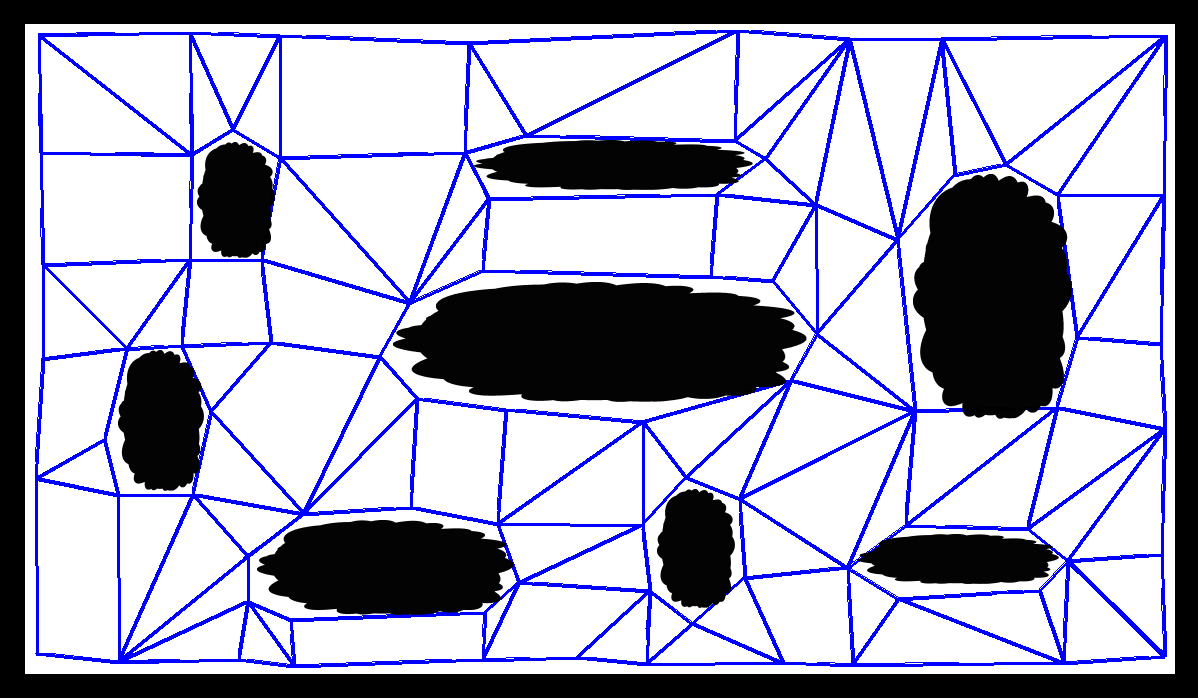
\includegraphics[scale=0.23]{figures/g1.png}
		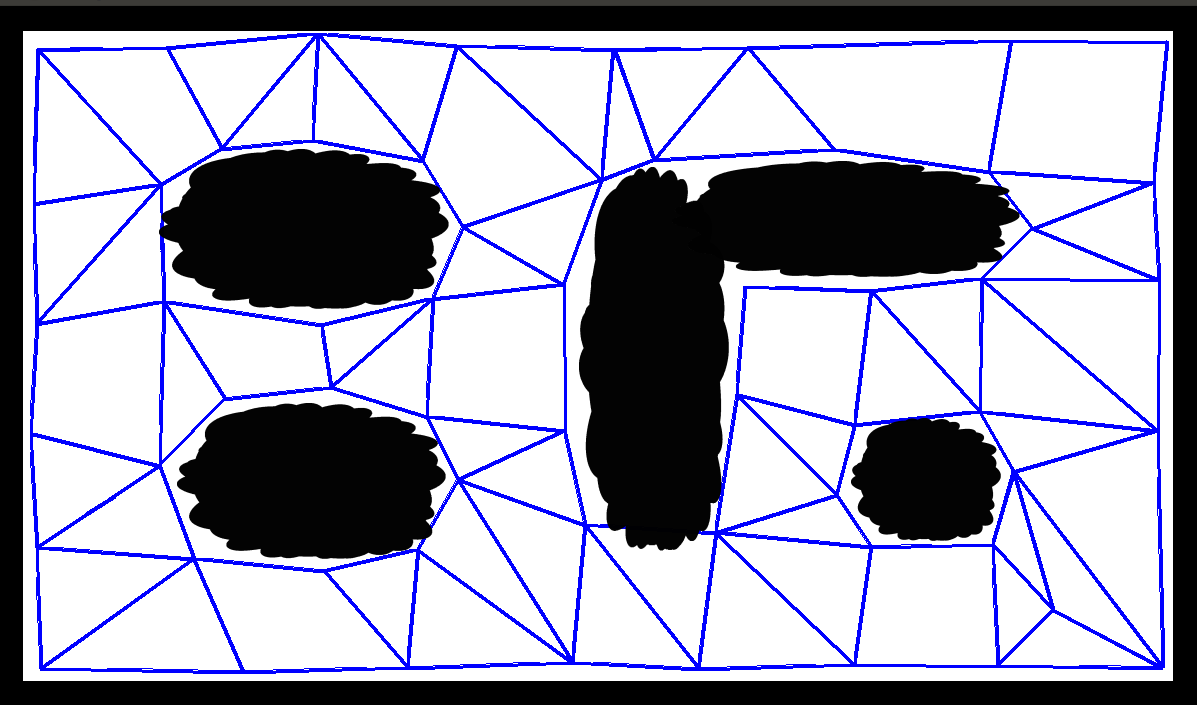
\includegraphics[scale=0.23]{figures/g2.png}
	\end{center}
	\caption{\label{fig:gs}
	     \textbf{Arriba:} Mapa 1 poligonalizado (60 pol\'igonos).
	     \textbf{Abajo:} Mapa 2 poligonalizado (85 pol\'igonos).
     }
\end{figure}
\end{comment}

Se utilizaron diversas topolog\'ias de grafos, para las cuales
se generan grafos aleatoriamente de distintos tamaños. Para cada
experimento se efect\'uan 100 disposiciones distintas de agentes
y del nodo objetivo. En los casos donde se referencia
que todos los agentes parten de la misma posici\'on inicial, \'esta es
com\'un para todos ellos, sin embargo, su disposici\'on es aleatoria.
Para cada uno de estos algoritmos se muestra el valor de emboscada
utilizando la m\'etrica originalmente propuesta y utilizando la
m\'etrica propuesta en el presente trabajo. Se prob\'o variar el
n\'umero de agentes con el fin de mostrar su impacto en el grado de emboscada.
Adem\'as, se muestran resultados con las dos instancias de mapas ($g1$ y $g2$)
presentadas en el trabajo previo \cite{FGC12} con 60 y 85 nodos
respectivamente. Estos mapas provienen de la poligonalizaci\'on de mapas
de juego en pol\'igonos. Este tipo de grafos son ampliamente utilizados
en juegos\cite{MF09}.

Para los experimentos con los grafos iniciales (g1 y g2), se mostr\'o
la efectividad de las tres variantes propuestas con respecto a \astar.
Adicionalmente, se evidencia en este y otros experimentos la mejora
al evaluar el grado de emboscada utilizando la m\'etrica nueva, dado
que la original subeval\'ua va\-rios casos de emboscada.
Los resultados de este experimento se pueden evidenciar en la tabla
\ref{tab:ambush_g}. Asimismo, en este y en los experimentos subsiguientes,
se puede apreciar como en los casos donde los agentes parten de una misma
posici\'on inicial, las diversas variantes de \ambush\ logran efectivamente
mejorar el grado de emboscada, incluso con un n\'umero bajo de agentes
involucrados.

\begin{table}
	\caption{Calidad de emboscada para grafos tipo Erd\H{o}s-R{\'e}nyi
	con \textbf{n} nodos, probabilidad de conexi\'on 0.7 y n\'umero de agentes
	(\textbf{\#}) ubicados en posiciones aleatorias distintas (arriba) y
	compartiendo la posici\'on inicial (abajo)}
	\label{tab:ambush_er}
	\centering
	\begin{small}
		\setlength{\tabcolsep}{4pt}
		\begin{tabular}{|c|c|cc|cc|cc|cc|}
			\hline
			\multirow{2}{*}{\textbf{n}} &
			\multirow{2}{*}{\textbf{\#}} &
			\multicolumn{2}{c|}{\textbf{\astar}} &
			\multicolumn{2}{c|}{\textbf{\ambush}} &
			\multicolumn{2}{c|}{\textbf{P}} &
			\multicolumn{2}{c|}{\textbf{SAR}}\\
			& & $\Phi$ & $\Phi^*$ & $\Phi$ & $\Phi^*$&
			$\Phi$ & $\Phi^*$& $\Phi$ & $\Phi^*$\\
			\hline
			\multirow{4}{*}{$10^2$}
			 & 2 & 0.39 & 0.98 & 0.41 & 1.00 & 0.41 & 1.00 & 0.41 & 1.00\\
			 & 5 & 0.32 & 0.93 & 0.35 & 0.98 & 0.35 & 0.98 & 0.35 & 0.98\\
			 & 10 & 0.34 & 0.88 & 0.38 & 0.95 & 0.38 & 0.95 & 0.38 & 0.95\\
			 & 20 & 0.49 & 0.89 & 0.53 & 0.94 & 0.53 & 0.94 & 0.53 & 0.94\\
			\hline
			\multirow{4}{*}{$10^3$}
			 & 2 & 0.50 & 1.00 & 0.50 & 1.00 & 0.50 & 1.00 & 0.50 & 1.00\\
			 & 5 & 0.43 & 0.96 & 0.45 & 0.99 & 0.45 & 0.99 & 0.45 & 0.99\\
			 & 10 & 0.42 & 0.92 & 0.47 & 0.99 & 0.47 & 0.99 & 0.47 & 0.99\\
			 & 20 & 0.40 & 0.82 & 0.47 & 0.94 & 0.47 & 0.94 & 0.47 & 0.94\\
			 \hline
			\multirow{4}{*}{$10^4$}
			 & 2 & 0.47 & 0.99 & 0.48 & 1.00 & 0.48 & 1.00 & 0.48 & 1.00\\
			 & 5 & 0.44 & 0.99 & 0.45 & 1.00 & 0.45 & 1.00 & 0.45 & 1.00\\
			 & 10 & 0.44 & 0.95 & 0.47 & 1.00 & 0.47 & 1.00 & 0.47 & 1.00\\
			 & 20 & 0.44 & 0.87 & 0.50 & 0.98 & 0.50 & 0.98 & 0.50 & 0.98\\
			 \hline
		\end{tabular}
		
		\bigskip
		\begin{tabular}{|c|c|cc|cc|cc|cc|}
			\hline
			\multirow{2}{*}{\textbf{n}} &
			\multirow{2}{*}{\textbf{\#}} &
			\multicolumn{2}{c|}{\textbf{\astar}} &
			\multicolumn{2}{c|}{\textbf{\ambush}} &
			\multicolumn{2}{c|}{\textbf{P}} &
			\multicolumn{2}{c|}{\textbf{SAR}}\\
			& & $\Phi$ & $\Phi^*$ & $\Phi$ & $\Phi^*$&
			$\Phi$ & $\Phi^*$& $\Phi$ & $\Phi^*$\\
			\hline
			\multirow{4}{*}{$10^2$}
			 & 2 & 0.43 & 0.68 & 0.69 & 0.94 & 0.69 & 0.94 & 0.69 & 0.94\\
			 & 5 & 0.27 & 0.52 & 0.59 & 0.92 & 0.59 & 0.92 & 0.60 & 0.92\\
			 & 10 & 0.25 & 0.52 & 0.54 & 0.96 & 0.54 & 0.96 & 0.54 & 0.96\\
			 & 20 & 0.20 & 0.49 & 0.48 & 0.93 & 0.48 & 0.93 & 0.47 & 0.92\\
			\hline
			\multirow{4}{*}{$10^3$}
			 & 2 & 0.40 & 0.63 & 0.74 & 0.97 & 0.74 & 0.97 & 0.74 & 0.97\\
			 & 5 & 0.15 & 0.52 & 0.56 & 0.93 & 0.56 & 0.93 & 0.56 & 0.93\\
			 & 10 & 0.09 & 0.47 & 0.49 & 0.93 & 0.49 & 0.93 & 0.48 & 0.91\\
			 & 20 & 0.06 & 0.46 & 0.42 & 0.93 & 0.42 & 0.93 & 0.39 & 0.89\\
			 \hline
			\multirow{4}{*}{$10^4$}
			 & 2 & 0.22 & 0.81 & 0.38 & 0.97 & 0.38 & 0.97 & 0.38 & 0.97\\
			 & 5 & 0.10 & 0.64 & 0.39 & 0.92 & 0.39 & 0.92 & 0.39 & 0.92\\
			 & 10 & 0.05 & 0.65 & 0.32 & 0.94 & 0.32 & 0.94 & 0.32 & 0.94\\
			 & 20 & 0.02 & 0.69 & 0.22 & 0.96 & 0.22 & 0.96 & 0.20 & 0.94\\
			 \hline
		\end{tabular}
	\end{small}
\end{table}


Para demostrar la necesidad de la creaci\'on de esta nueva m\'etrica,
se procedi\'o a probar la efectividad del algoritmo utilizando grafos
con poca diversidad posible de caminos, en los cuales, no es posible
generar emboscadas totales en muchos casos. Para esto, se utilizaron
grafos tipo langosta (Lobster graphs) \cite{Gal09} y grafos generados
bajo el modelo propuesto por Erd\H{o}s y R{\'e}nyi (grafos binomiales)
\cite{ER59}, siendo \'estos convertidos a grafos dirigidos con el fin de
reducir el n\'umero de componentes fuertemente conexas. Los experimentos sobre
grafos tipo langosta representan el peor caso para la m\'etrica originalmente
propuesta; dado que estos son \'arboles, existe s\'olo un camino entre
cualquier par de nodos, por lo que no es posible cubrir aquellos nodos
es\-ca\-pa\-to\-ria sin pasar por el nodo objetivo. En la tabla
\ref{tab:ambush_lobster} se muestran los resultados obtenidos utilizando
este tipo de grafos.
An\'alogamente, en la tabla \ref{tab:ambush_er} se muestran los resultados
para el modelo Erd{\H{o}s-R{\'e}nyi. Para este tipo de grafos, dada la
e\-xis\-ten\-cia de m\'ultiples caminos entre un par de nodos, no s\'olo se
evidencia una mejora de la nueva m\'etrica con respecto a la anterior, sino
tambi\'en de las variantes de \ambush\ con respecto a \astar. La mejora
aportada por \ambush\ parece casi imperceptible al ser estudiada
con la m\'etrica original, sin embargo, al ser analizado con la nueva
m\'etrica, se hace notar que el grado de emboscada alcanzado tiende a ser
el m\'aximo posible.

\begin{table}
	\caption{Calidad de emboscada para grafos tipo grilla cuadrada
	utilizando distinto tamaño de grilla (\textbf{n x n}) y n\'umero de agentes
	(\textbf{\#}) ubicados en posiciones aleatorias distintas (arriba) y
	compartiendo la posici\'on inicial (abajo)}
	\label{tab:ambush_grid}
	\centering
	\begin{small}
		\setlength{\tabcolsep}{4pt}
		\begin{tabular}{|c|c|cc|cc|cc|cc|}
			\hline
			\multirow{2}{*}{\textbf{n}} &
			\multirow{2}{*}{\textbf{\#}} &
			\multicolumn{2}{c|}{\textbf{\astar}} &
			\multicolumn{2}{c|}{\textbf{\ambush}} &
			\multicolumn{2}{c|}{\textbf{P}} &
			\multicolumn{2}{c|}{\textbf{SAR}}\\
			& & $\Phi$ & $\Phi^*$ & $\Phi$ & $\Phi^*$&
			$\Phi$ & $\Phi^*$& $\Phi$ & $\Phi^*$\\
			\hline
			\multirow{4}{*}{10}
			 & 2 & 0.88 & 0.89 & 0.98 & 0.98 & 0.98 & 0.98 & 0.98 & 0.98\\
			 & 5 & 0.65 & 0.65 & 0.95 & 0.95 & 0.95 & 0.95 & 0.95 & 0.95\\
			 & 10 & 0.72 & 0.72 & 0.92 & 0.92 & 0.92 & 0.92 & 0.93 & 0.93\\
			 & 20 & 0.83 & 0.83 & 0.96 & 0.96 & 0.96 & 0.96 & 0.96 & 0.96\\
			\hline
			\multirow{4}{*}{20}
			 & 2 & 0.89 & 0.90 & 1.00 & 1.00 & 1.00 & 1.00 & 1.00 & 1.00\\
			 & 5 & 0.65 & 0.65 & 0.98 & 0.98 & 0.98 & 0.98 & 0.97 & 0.98\\
			 & 10 & 0.66 & 0.66 & 0.96 & 0.96 & 0.96 & 0.96 & 0.96 & 0.96\\
			 & 20 & 0.78 & 0.78 & 0.97 & 0.97 & 0.97 & 0.97 & 0.97 & 0.97\\
			 \hline
			\multirow{4}{*}{100}
			 & 2 & 0.89 & 0.89 & 1.00 & 1.00 & 1.00 & 1.00 & 1.00 & 1.00\\
			 & 5 & 0.68 & 0.68 & 1.00 & 1.00 & 1.00 & 1.00 & 1.00 & 1.00\\
			 & 10 & 0.58 & 0.58 & 0.99 & 0.99 & 0.99 & 0.99 & 0.99 & 0.99\\
			 & 20 & 0.74 & 0.74 & 0.99 & 0.99 & 0.99 & 0.99 & 0.99 & 0.99\\
			 \hline
		\end{tabular}
		
		\bigskip
		\begin{tabular}{|c|c|cc|cc|cc|cc|}
			\hline
			\multirow{2}{*}{\textbf{n}} &
			\multirow{2}{*}{\textbf{\#}} &
			\multicolumn{2}{c|}{\textbf{\astar}} &
			\multicolumn{2}{c|}{\textbf{\ambush}} &
			\multicolumn{2}{c|}{\textbf{P}} &
			\multicolumn{2}{c|}{\textbf{SAR}}\\
			& & $\Phi$ & $\Phi^*$ & $\Phi$ & $\Phi^*$&
			$\Phi$ & $\Phi^*$& $\Phi$ & $\Phi^*$\\
			\hline
			\multirow{4}{*}{10}
			 & 2 & 0.50 & 0.49 & 0.98 & 0.98 & 0.98 & 0.98 & 0.98 & 0.98\\
			 & 5 & 0.20 & 0.20 & 0.89 & 0.89 & 0.89 & 0.89 & 0.89 & 0.89\\
			 & 10 & 0.16 & 0.16 & 0.89 & 0.89 & 0.89 & 0.89 & 0.83 & 0.83\\
			 & 20 & 0.16 & 0.16 & 0.91 & 0.91 & 0.91 & 0.91 & 0.82 & 0.82\\
			\hline
			\multirow{4}{*}{20}
			 & 2 & 0.50 & 0.49 & 0.99 & 0.99 & 0.99 & 0.99 & 0.99 & 0.99\\
			 & 5 & 0.20 & 0.20 & 0.96 & 0.96 & 0.96 & 0.96 & 0.97 & 0.97\\
			 & 10 & 0.14 & 0.14 & 0.97 & 0.97 & 0.97 & 0.97 & 0.93 & 0.93\\
			 & 20 & 0.14 & 0.14 & 0.96 & 0.96 & 0.96 & 0.96 & 0.93 & 0.93\\
			 \hline
			\multirow{4}{*}{100}
			 & 2 & 0.50 & 0.50 & 1.00 & 1.00 & 1.00 & 1.00 & 1.00 & 1.00\\
			 & 5 & 0.20 & 0.20 & 1.00 & 1.00 & 1.00 & 1.00 & 1.00 & 1.00\\
		  	 & 10 & 0.13 & 0.13 & 0.99 & 0.99 & 0.99 & 0.99 & 0.98 & 0.98\\
			 & 20 & 0.13 & 0.13 & 1.00 & 0.99 & 1.00 & 0.99 & 0.98 & 0.98\\
			 \hline
		\end{tabular}
	\end{small}
\end{table}


\begin{table}
	\caption{Calidad de emboscada para grafos tipo Watts-Strotgatz small-world
	utilizando distinto n\'umero de nodos, 10 vecinos cercanos, probabilidad
	de reconexi\'on 0.5 y n\'umero de agentes
	(\textbf{\#}) ubicados en posiciones aleatorias distintas (arriba) y
	compartiendo la posici\'on inicial (abajo)}
	\label{tab:ambush_watts}
	\centering
	\begin{small}
		\setlength{\tabcolsep}{4pt}
		\begin{tabular}{|c|c|cc|cc|cc|cc|}
			\hline
			\multirow{2}{*}{\textbf{n}} &
			\multirow{2}{*}{\textbf{\#}} &
			\multicolumn{2}{c|}{\textbf{\astar}} &
			\multicolumn{2}{c|}{\textbf{\ambush}} &
			\multicolumn{2}{c|}{\textbf{P}} &
			\multicolumn{2}{c|}{\textbf{SAR}}\\
			& & $\Phi$ & $\Phi^*$ & $\Phi$ & $\Phi^*$&
			$\Phi$ & $\Phi^*$& $\Phi$ & $\Phi^*$\\
			\hline
			\multirow{4}{*}{$10^2$}
			 & 2 & 0.94 & 0.94 & 1.00 & 0.99 & 1.00 & 0.99 & 1.00 & 0.99\\
			 & 5 & 0.77 & 0.78 & 0.96 & 0.98 & 0.96 & 0.98 & 0.96 & 0.98\\
			 & 10 & 0.68 & 0.68 & 0.97 & 0.97 & 0.97 & 0.97 & 0.97 & 0.97\\
			 & 20 & 0.84 & 0.84 & 1.00 & 1.00 & 1.00 & 1.00 & 1.00 & 1.00\\
			\hline
			\multirow{4}{*}{$10^3$}
			 & 2 & 0.95 & 0.95 & 1.00 & 1.00 & 1.00 & 1.00 & 1.00 & 1.00\\
			 & 5 & 0.79 & 0.79 & 1.00 & 1.00 & 1.00 & 1.00 & 1.00 & 1.00\\
			 & 10 & 0.66 & 0.67 & 1.00 & 1.00 & 1.00 & 1.00 & 1.00 & 1.00\\
			 & 20 & 0.86 & 0.86 & 1.00 & 1.00 & 1.00 & 1.00 & 1.00 & 1.00\\
			 \hline
			\multirow{4}{*}{$10^4$}
			 & 2 & 0.95 & 0.95 & 1.00 & 1.00 & 1.00 & 1.00 & 1.00 & 1.00\\
			 & 5 & 0.82 & 0.82 & 1.00 & 1.00 & 1.00 & 1.00 & 1.00 & 1.00\\
			 & 10 & 0.68 & 0.68 & 1.00 & 1.00 & 1.00 & 1.00 & 1.00 & 1.00\\
			 & 20 & 0.87 & 0.87 & 1.00 & 1.00 & 1.00 & 1.00 & 1.00 & 1.00\\
			 \hline
		\end{tabular}
		
		\bigskip
		\begin{tabular}{|c|c|cc|cc|cc|cc|}
			\hline
			\multirow{2}{*}{\textbf{n}} &
			\multirow{2}{*}{\textbf{\#}} &
			\multicolumn{2}{c|}{\textbf{\astar}} &
			\multicolumn{2}{c|}{\textbf{\ambush}} &
			\multicolumn{2}{c|}{\textbf{P}} &
			\multicolumn{2}{c|}{\textbf{SAR}}\\
			& & $\Phi$ & $\Phi^*$ & $\Phi$ & $\Phi^*$&
			$\Phi$ & $\Phi^*$& $\Phi$ & $\Phi^*$\\
			\hline
			\multirow{4}{*}{$10^2$}
			 & 2 & 0.50 & 0.49 & 0.93 & 0.93 & 0.93 & 0.93 & 0.93 & 0.93\\
			 & 5 & 0.20 & 0.20 & 0.89 & 0.89 & 0.89 & 0.89 & 0.89 & 0.89\\
			 & 10 & 0.11 & 0.11 & 0.89 & 0.89 & 0.89 & 0.89 & 0.88 & 0.88\\
			 & 20 & 0.10 & 0.10 & 0.80 & 0.80 & 0.80 & 0.80 & 0.78 & 0.78\\
			\hline
			\multirow{4}{*}{$10^3$}
			 & 2 & 0.50 & 0.49 & 0.99 & 0.98 & 0.99 & 0.98 & 0.99 & 0.98\\
			 & 5 & 0.20 & 0.20 & 0.99 & 0.99 & 0.99 & 0.99 & 0.99 & 0.99\\
			 & 10 & 0.11 & 0.11 & 0.99 & 0.99 & 0.99 & 0.99 & 0.99 & 0.99\\
			 & 20 & 0.10 & 0.10 & 1.00 & 1.00 & 1.00 & 1.00 & 1.00 & 1.00\\
			 \hline
			\multirow{4}{*}{$10^4$}
			 & 2 & 0.50 & 0.50 & 1.00 & 0.99 & 1.00 & 0.99 & 1.00 & 0.99\\
			 & 5 & 0.20 & 0.20 & 1.00 & 1.00 & 1.00 & 1.00 & 1.00 & 1.00\\
			 & 10 & 0.11 & 0.11 & 0.99 & 0.99 & 0.99 & 0.99 & 1.00 & 1.00\\
			 & 20 & 0.11 & 0.11 & 1.00 & 1.00 & 1.00 & 1.00 & 1.00 & 1.00\\
			 \hline
		\end{tabular}
	\end{small}
\end{table}


\begin{table}
	\caption{Calidad de emboscada para grafos tipo Navigable Small-World 
	utilizando conecciones de corto alcance de tamaño unitario y cinco conexiones
	de largo alcance por nodo, n\'umero de agentes (\textbf{\#}) ubicados en
	posiciones aleatorias distintas (arriba) y compartiendo la posici\'on
	inicial (abajo)}
	\label{tab:ambush_nswg}
	\centering
	\begin{small}
		\setlength{\tabcolsep}{4pt}
		\begin{tabular}{|c|c|cc|cc|cc|cc|}
			\hline
			\multirow{2}{*}{\textbf{n}} &
			\multirow{2}{*}{\textbf{\#}} &
			\multicolumn{2}{c|}{\textbf{\astar}} &
			\multicolumn{2}{c|}{\textbf{\ambush}} &
			\multicolumn{2}{c|}{\textbf{P}} &
			\multicolumn{2}{c|}{\textbf{SAR}}\\
			& & $\Phi$ & $\Phi^*$ & $\Phi$ & $\Phi^*$&
			$\Phi$ & $\Phi^*$& $\Phi$ & $\Phi^*$\\
			\hline
			\multirow{4}{*}{$10$}
			 & 2 & 0.93 & 0.94 & 0.99 & 1.00 & 0.99 & 1.00 & 0.99 & 1.00\\
			 & 5 & 0.79 & 0.79 & 0.96 & 0.97 & 0.96 & 0.97 & 0.97 & 0.97\\
			 & 10 & 0.66 & 0.68 & 0.93 & 0.96 & 0.93 & 0.96 & 0.93 & 0.96\\
			 & 20 & 0.77 & 0.81 & 0.96 & 1.00 & 0.96 & 1.00 & 0.96 & 1.00\\
			\hline
			\multirow{4}{*}{$20$}
			 & 2 & 0.93 & 0.94 & 0.99 & 1.00 & 0.99 & 1.00 & 0.99 & 1.00\\
			 & 5 & 0.85 & 0.85 & 1.00 & 1.00 & 1.00 & 1.00 & 1.00 & 1.00\\
			 & 10 & 0.71 & 0.72 & 0.99 & 0.99 & 0.99 & 0.99 & 0.99 & 0.99\\
			 & 20 & 0.77 & 0.78 & 0.99 & 1.00 & 0.99 & 1.00 & 0.99 & 1.00\\
			 \hline
			\multirow{4}{*}{$50$}
			 & 2 & 0.95 & 0.95 & 1.00 & 1.00 & 1.00 & 1.00 & 1.00 & 1.00\\
			 & 5 & 0.85 & 0.85 & 1.00 & 1.00 & 1.00 & 1.00 & 1.00 & 1.00\\
			 & 10 & 0.73 & 0.73 & 1.00 & 1.00 & 1.00 & 1.00 & 1.00 & 1.00\\
			 & 20 & 0.77 & 0.78 & 0.99 & 1.00 & 0.99 & 1.00 & 0.99 & 1.00\\
			 \hline
			\multirow{4}{*}{$100$}
			 & 2 & 0.98 & 0.98 & 1.00 & 1.00 & 1.00 & 1.00 & 1.00 & 1.00\\
			 & 5 & 0.84 & 0.84 & 1.00 & 1.00 & 1.00 & 1.00 & 1.00 & 1.00\\
			 & 10 & 0.72 & 0.72 & 1.00 & 1.00 & 1.00 & 1.00 & 1.00 & 1.00\\
			 & 20 & 0.77 & 0.77 & 1.00 & 1.00 & 1.00 & 1.00 & 1.00 & 1.00\\
			 \hline
		\end{tabular}
		
		\bigskip
		\begin{tabular}{|c|c|cc|cc|cc|cc|}
			\hline
			\multirow{2}{*}{\textbf{n}} &
			\multirow{2}{*}{\textbf{\#}} &
			\multicolumn{2}{c|}{\textbf{\astar}} &
			\multicolumn{2}{c|}{\textbf{\ambush}} &
			\multicolumn{2}{c|}{\textbf{P}} &
			\multicolumn{2}{c|}{\textbf{SAR}}\\
			& & $\Phi$ & $\Phi^*$ & $\Phi$ & $\Phi^*$&
			$\Phi$ & $\Phi^*$& $\Phi$ & $\Phi^*$\\
			\hline
			\multirow{4}{*}{$10$}
			& 2 & 0.50 & 0.50 & 0.94 & 0.94 & 0.94 & 0.94 & 0.94 & 0.94\\
			& 5 & 0.20 & 0.21 & 0.95 & 0.96 & 0.95 & 0.96 & 0.95 & 0.96\\
			& 10 & 0.10 & 0.11 & 0.85 & 0.86 & 0.85 & 0.86 & 0.85 & 0.86\\
			& 20 & 0.09 & 0.10 & 0.92 & 0.96 & 0.92 & 0.96 & 0.84 & 0.88\\
			\hline
			\multirow{4}{*}{$20$}
			& 2 & 0.50 & 0.50 & 0.99 & 0.99 & 0.99 & 0.99 & 0.99 & 0.99\\
			& 5 & 0.20 & 0.20 & 0.98 & 0.98 & 0.98 & 0.98 & 0.98 & 0.98\\
			& 10 & 0.10 & 0.10 & 0.93 & 0.94 & 0.93 & 0.94 & 0.93 & 0.94\\
			& 20 & 0.08 & 0.08 & 0.98 & 0.99 & 0.98 & 0.99 & 0.97 & 0.99\\
			\hline
			\multirow{4}{*}{$50$}
			& 2 & 0.50 & 0.50 & 1.00 & 1.00 & 1.00 & 1.00 & 1.00 & 1.00\\
			& 5 & 0.20 & 0.20 & 0.99 & 0.99 & 0.99 & 0.99 & 0.99 & 0.99\\
			& 10 & 0.10 & 0.10 & 0.99 & 0.99 & 0.99 & 0.99 & 0.99 & 0.99\\
			& 20 & 0.08 & 0.08 & 1.00 & 1.00 & 1.00 & 1.00 & 1.00 & 1.00\\
			 \hline
			\multirow{4}{*}{$100$}
			& 2 & 0.50 & 0.50 & 1.00 & 1.00 & 1.00 & 1.00 & 1.00 & 1.00\\
			& 5 & 0.20 & 0.20 & 1.00 & 1.00 & 1.00 & 1.00 & 1.00 & 1.00\\
			& 10 & 0.10 & 0.10 & 1.00 & 1.00 & 1.00 & 1.00 & 1.00 & 1.00\\
			& 20 & 0.07 & 0.07 & 0.99 & 0.99 & 0.99 & 0.99 & 0.98 & 0.98\\
			\hline
		\end{tabular}
	\end{small}
\end{table}


Los dem\'as grafos utilizados son de varios tipos provenientes de la
literatura. El primer tipo de grafos generados explorado son los grafos
en grilla cuadrada con 8-conectividad, los cuales son muy comunes en el
desarrollo de juegos debido a la eficacia en la determinaci\'on de caminos
y en la ubicaci\'on del agente en una de las ca\-si\-llas \cite{MF09}.
Los resultados de este experimento se pueden apreciar en la tabla
\ref{tab:ambush_grid}. A medida que el grafo se hace m\'as grande, la
calidad media de emboscada se hace mayor, sin embargo, a\'un en grafos
pequeños se muestra que la emboscada se alcanza efectivamente. Para este
tipo de grafos ambas m\'etricas reportan los mismos valores dado que la
grilla se encuentra completamente conectada, siendo posible alcanzar a
cualquier nodo por m\'as de una v\'ia. De esta forma,
ambos conjuntos, el de predecesores y el de asociaci\'on de agentes a
nodos son el mismo, por lo que el factor de normalizaci\'on act\'ua de la
misma forma en ambas m\'etricas. Este fen\'omeno no se aprecia en los otros
tipos de grafos estudiados.

Seguidamente se experiment\'o con grafos con propiedad de mundo-pequeño
(Small-World Networks) \cite{WS98}. En este tipo de grafos
la mayor\'ia de los nodos no son vecinos de los dem\'as, sin embargo,
la mayor\'ia son alcanzables por cualquier otro utilizando caminos con
un n\'umero corto de pasos. Este tipo de grafos podr\'ian ser dif\'iciles
para un m\'etodo como \ambush\ debido a esta propiedad, al no ofrecer suficiente
distancia para que los agentes se alejen imposibilitando as\'i alcanzar la
emboscada. Sin embargo, en las tablas \ref{tab:ambush_watts} y \ref{tab:ambush_nswg}
se muestra que el algoritmo es capaz de so\-bre\-lle\-var esta situaci\'on y lograr
emboscadas perfectas en muchos de los casos. Los tipos de grafos con esta
propiedad es\-tu\-dia\-dos son los propuestos por Watts y Strogatz \cite{WS98}
y el propuesto por Kleinberg \cite{Kle00}.

Finalmente, se realizaron experimentos con el modelo de grafos propuesto
por Dorogovtsev y Mendes \cite{DM02}. El cual produce grafos planares,
similares a los utilizados en el \'area de inter\'es. Bajo este tipo
de grafos, si bien el grado de emboscada alcanzado fue menor con respecto
a los otros tipos utilizados, se mostr\'o un incremento significativo
de este con respecto al algoritmo base probado \astar.